% !Mode:: "TeX:UTF-8"
\chapter{中微子物理}

中微子一直是粒子物理学中一个非常有趣且受到广泛关注的研究方向。
它们属于标准模型中的轻子,质量很小,并且与其他物质的相互作用非常微弱,
让我们很难去直接观察到它们的存在。不过,研究中微子对理解宇宙的起源和演变、
以及基本粒子之间的关系都非常重要。它们在宇宙中扮演着重要角色,
不仅参与核反应和高能宇宙射线的产生,还可能在宇宙的膨胀和
冷却过程中起到一定的作用。


本章节主要介绍中微子物理,\ref{sec:neutrino_discovery}节回顾了中微子的发现历程,
\ref{sec:neutrino_oscillation}节简要介绍了中微子振荡现象,
\ref{sec:neutrino_mass}节介绍了中微子质量以及
\ref{sec:double_beta_decay}节介绍了双贝塔衰变的相关问题。

\section{中微子的发现历程}\label{sec:neutrino_discovery}

1914年,Chadwick J.在研究$\beta$衰变过程中发现了一个令人困惑的问题:$\beta$衰变中电子的能量呈现出连续分布的谱线,而非单一常数值。
这一现象与当时理论预期的单一能量释放过程不符。
为了解释这一现象,1930年,Pauli W.提出了一个假设:在$\beta$衰变过程中,除了电子外,还存在一个未被观测到的粒子参与其中,
这个粒子后来被称为"中微子"。
1934年,Fermi E.提出了中微子与电子的相互作用理论,并正式将其命名为"中微子"。
1942年王淦昌首先提出使用电子俘获的方法来探测中微子,
而直到1956年,Reines F.和Cowans C.才首次在实验中成功探测到了中微子,证实了它们的存在。\cite{science.124.3212.103}
到1962年,Lederman L.等人发现中微子不止一种,除了之前发现的电子中微子外,他们还发现了
$\mu$子中微子。当第三种轻子$\tau$子于1975年被发现后,科学家们又在2000年
证实了第三种中微子——$\tau$中微子的存在。这三种中微子具有不同的味道,分别对应三种轻子:电子、$\mu$子和$\tau$子。

\section{中微子振荡}\label{sec:neutrino_oscillation}

由超级神冈对于大气中微子中穿过地球的$\mu$子中微子缺失测量的结果
和由SNO实验通过对太阳中微子的带电流和中性流的测量对
"太阳中微子消失之谜"的解答可以看出,中微子在传播过程中会发生振荡现象,
即中微子的三种味道会在其传播过程相互转化。这意味着中微子是具有内禀时钟,
从而得出了与标准模型的预测完全不同的结果——中微子具有静止质量。
中微子振荡的现象可以用一个简单的模型来描述。现在有三种我们可以探测到的中微子,分别是电子中微子$\nu_e$、$\mu$子中微子$\nu_\mu$和$\tau$子中微子$\nu_\tau$。
那么根据薛定谔方程,考虑平面波,在真空中,从一种味道的中微子$\ket{\nu_\alpha}$到另一种味道$\ket{\nu_\beta}$的转化的概率是:\footnote{这里考虑了相对论效应,且由于中微子能量$E$远大于中微子静止质量$m$,故可以
在自然单位制下近似认为$E=\bar{p}$,$\bar{p}$为中微子的平均动量。}

\begin{equation}
    \label{oscillation}
    P_{\nu_\alpha \to \nu_\beta} = \delta_{\alpha\beta} - 4\sum_{i>j=1} \mathbf{Re} (K_{\alpha\beta,ij}) \sin^2\left(\frac{\Delta m_{ij}^2 L}{4E}\right) - 4 \sum_{i>j=1} \mathbf{Im} (K_{\alpha\beta,ij}) \sin\left (\frac{\Delta m_{ij}^2 L}{2E}\right) 
\end{equation}

其中
\begin{equation}
    K_{\alpha\beta,ij} = U_{\alpha i} U_{\beta i}^* U_{\alpha j} U_{\beta j}^*
\end{equation}

$\Delta m^2_{ij}$为质量本征态$\ket{\nu_i}$与质量本征态$\ket{\nu_j}$的平方差值,$L=x=ct$为中微子源到探测器的距
离。$U$为PMNS矩阵:

\begin{equation}
    \ket{\nu_\alpha} = U_{PMNS}\ket{\nu_i}\quad \alpha=e,\mu,\tau;i=1,2,3
\end{equation}

\begin{equation}
    \label{PMNS}
    U = \begin{pmatrix}
        1 & 0 & 0 \\
        0 & c_{23} & s_{23} \\
        0 & -s_{23} & c_{23}
    \end{pmatrix}
    \begin{pmatrix}
        c_{13} & 0 & s_{13} e^{-i\delta} \\
        0 & 1 & 0 \\
        -s_{13} e^{i\delta} & 0 & c_{13}
    \end{pmatrix}
    \begin{pmatrix}
        c_{12} & s_{12} & 0 \\
        -s_{12} & c_{12} & 0 \\
        0 & 0 & 1
    \end{pmatrix}
\end{equation}

\bigskip

其中$s_{ij}=\sin\theta_{ij}$,$c_{ij}=\cos\theta_{ij}$ $ (i,j=1,2,3) $,
$\theta_{ij}$为混合角,$\delta$为CP相位。这是对于Dirac中微子
的PMNS (Pontecorvo–Maki–Nakagawa–Sakata) 矩阵,而对于Majorana中微子,会引入额外的两个相位参数:
\begin{equation}
    U=U_{PMNS}·\text{diag} (1,e^{i\alpha_1},e^{i\alpha_2}) 
\end{equation}
但是不影响整体的中微子
振荡,因为取模之后这些因子都被消去了。

\section{中微子质量}\label{sec:neutrino_mass}
中微子振荡的发现打开了中微子研究的新领域,
其中最重要的问题是,既然中微子具有质量,
那么它们的质量是多少?以及它们的质量是如何产生的呢?
一般认为,中微子质量有两种来源:一是通过希格斯机制,
类似于其他费米子。另外一种猜测是中微子可能是一直没有被发现
的Majorana费米子,即中微子的反粒子是它本身。对于Majorana
中微子,需要超出标准模型的理论进行解释。一个最吸引人的模型
是所谓的"翘翘板"机制,其引入了具有超大Majorana质量项的右手中微子,
从而可以获得一个超大的质量本征值和一个很小的质量本征值。


考虑左手中微子和超大质量的右手中微子以及对应的反中微子通过Dirac质量项和Majorana
质量项的耦合,其拉格朗日量为\cite{zuber2020neutrino}\footnote{式中$h.c.$代表厄米共轭}:
\begin{align}
    \label{Lagrangian_D-M}
    2\mathcal{L} &= m_D (\bar{\nu}_L N_R + \bar{N}_L^c \nu_R^c) + m_L \bar{\nu}_L \nu_R^c + m_R \bar{N}_L^c N_R + h.c. \\
    &= (\bar{\nu}_L, \bar{N}_L^c) 
    \begin{pmatrix}
    m_L & m_D \\
    m_D & m_R
    \end{pmatrix}
    \begin{pmatrix}
    \nu_R^c \\
    N_R
    \end{pmatrix}
    + h.c.
\end{align}
其中$\nu_L$为左手中微子,$\nu^c_R$为其对应的反中微子,$m_L$为其质量
$N_R$为引入的超大质量中微子,$N^c_L$为其对应的反中微子。$m_R$为其质量。
$m_D$为Dirac质量项,$m_R$为Majorana质量项。在标准模型中,
Majorana质量项不能出现,因为它是非规范不变的。
对于刚才提到的最简单的“翘翘板”机制,我们只需要令$m_L=0$,$m_R\gg m_D$,
则我们得到了两个质量本征态:
\begin{equation}
    m_\nu = m_1 = \frac{m^2_D}{m_R} \quad m_N = m_2
    = m_R\left(1+\frac{m^2_D}{m^2_R}\right) \approx m_R
\end{equation}


    
图\ref{DMscheme}是一个费米场,轻子以及中微子通过Dirac质量和Majorana质量耦合的示意图。
 (a) 为费米场的质量产生机制, (b) 为电子的质量产生机制, (c) 为"翘翘板"机制下中微子的质量产生机制,即上面的分析。

\begin{figure}[htbp]
    \centering
\begin{tikzpicture}[scale=1.2, every node/.style={font=\small}, >=Stealth]

    % Diagram (a) 

    \node[left] at (-1,2) {$\psi_L$};
    \node[left] at (-1,0) {$ (\psi_R) ^c$};
    \node[right] at (1,2) {$ (\psi_L) ^c$};
    \node[right] at (1,0) {$\psi_R$};
    \node at (0,-0.8) { (a) };

    \draw[<->] (-1,2) -- (1,2) node[midway, above] {Majorana};
    \draw[<->] (-1,0) -- (1,0) node[midway, below] {Majorana};
    \draw[->] (-0.2,0.8) -- (-1,0.2) ;
    \draw[->] (0.2,1.2) -- (1,1.8) ;
    \draw[<-] (-1,1.8) -- (-0.2,1.2) ;
    \draw[<-] (1,0.2) -- (0.2,0.8) ;
    \node at (0,1) {Dirac};
    
    % Diagram (b) 

    \node[left] at (3,2) {$e_L^-$};
    \node[left] at (3,0) {$e_L^+$};
    \node[right] at (5,2) {$e_R^+$};
    \node[right] at (5,0) {$e_R^-$};
    \node at (4,-0.8) { (b) };
    
    \draw[<->] (3,2) -- (5,2) node[midway, above] {$0$};
    \draw[<->] (3,0) -- (5,0) node[midway, below] {$0$};
    \draw[<-] (3,1.8) -- (3.8,1.2) ;
    \draw[<-] (5,1.8) -- (4.2,1.2) ;
    \draw[<-] (3,0.2) -- (3.8,0.8) ;
    \draw[<-] (5,0.2) -- (4.2,0.8) ;
    \node at (4,1) {$m_e$};
    
    % Diagram (c) 
    \node at (8,-0.8) { (c) };
    \node[left] at (7,2) {$\nu_L$};
    \node[left] at (7,0) {$ (\nu_R) ^c$};
    \node[right] at (9,2) {$ (\nu_L) ^c$};
    \node[right] at (9,0) {$\nu_R$};
    
    \draw[<->] (7,2) -- (9,2) node[midway, above] {$m_L^{\text{M}}$};
    \draw[<->] (7,0) -- (9,0) node[midway, below] {$m_R^{\text{M}}$};
    \draw[<-] (7,1.8) -- (7.8,1.2) ;
    \draw[<-] (9,1.8) -- (8.2,1.2) ;
    \draw[<-] (7,0.2) -- (7.8,0.8) ;
    \draw[<-] (9,0.2) -- (8.2,0.8) ;
    \node at (8,1) {$m^{\text{D}}$};
\end{tikzpicture}
\figcaption{费米场,电子,中微子通过Dirac质量和Majorana质量耦合的示意图\cite{zuber2020neutrino}}
\label{DMscheme}
\end{figure}


\section{双贝塔衰变}\label{sec:double_beta_decay}

$\beta\beta$ (Double Beta Decay,双贝塔衰变) 
是一种非常罕见的放射性衰变过程。在这种衰变中,原子核内的两个中子
 (或质子) 同时转变为两个质子 (或中子) ,并释放出两个电子 (或正电子) 
以及可能的中微子。

这个过程之所以受到关注,是因为它只发生在那些单贝塔衰变
 (一个中子转变为一个质子,释放一个电子和一个反中微子) 在能量上被
禁止或者因为角动量选择定则而被高度压抑的原子核中。换句话说,
如果一个原子核满足
\begin{equation}
    m (Z, A)  > m (Z+2, A)  \quad \quad m (Z,A)  < m (Z+1, A) 
\end{equation}    
那么它就可能经历$\beta\beta$。$\beta\beta$主要有两种模式:$2\nu\beta\beta$  (Two-neutrino double beta decay,双中微子双贝塔衰变) 
和$0\nu\beta\beta$  (Neutrinoless double beta decay,无中微子双贝塔衰变) 。

\subsection{2$\nu\beta\beta$}

    $2\nu\beta\beta$ 是标准模型框架中允许的过程。原子核内的两个中子转变为两个质子,
    同时释放出两个电子和两个电子反中微子  ($\bar{\nu}_e$) 。
    反应式可以写为:
    \begin{equation}
         (A, Z)  \rightarrow  (A, Z+2)  + 2e^{-} + 2\bar{\nu}_e
    \end{equation}
    这个过程遵守轻子数守恒定律 (初始轻子数为0,
    末态轻子数为 $2 \times  (+1)  + 2 \times  (-1)  = 0$) 。
    这一理论首先被Goeppert M.提出\cite{PhysRev.48.512},
    $2\nu\beta\beta$ 衰变已经被实验明确观测到,其半衰期极长,
    通常在 $10^{18}$ 到 $10^{21}$ 年的量级或更长\cite{ParticleDataGroup:2024cfk}。

    
$\beta\beta$的半衰期  ($T_{1/2}$)  可以通过以下公式描述:

对于 $2\nu\beta\beta$:
    \begin{equation}
        [ T^{2\nu}_{1/2} ]^{-1} = G^{2\nu} (Q, Z)  | M^{2\nu} |^2
    \end{equation}
    其中$T^{2\nu}_{1/2}$ 是 $2\nu\beta\beta$ 衰变的半衰期。
    $G^{2\nu} (Q, Z) $ 是可精确计算的相空间因子 (Phase Space Factor) ,它依赖于衰变能量 $Q$ 和原子核的电荷数 $Z$。
    $M^{2\nu}$ 是核矩阵元 (Nuclear Matrix Element, NME) ,它的计算高度依赖于核物理模型,是理论计算中的主要不确定性来源。



\subsection{$0\nu\beta\beta$}

$0\nu\beta\beta$是一个尚未被实验发现的极其稀有的过程。这个反应包括了
    原子核内的两个中子转变为两个质子,只释放出两个电子,而没有中微子被释放出来。
    反应式可以写为:
    \begin{equation}
         (A, Z)  \rightarrow  (A, Z+2)  + 2e^{-}
    \end{equation}
    这个过程违反了轻子数守恒定律  ($\Delta L = +2$) 。它的发生需要满足两个关键条件:
    \begin{enumerate}
        \item 中微子是Majorana粒子,即中微子和它的反粒子是同一种粒子  ($\nu = \bar{\nu}$) 。
        \item 中微子具有非零的质量。
    \end{enumerate}
    在这个模型中,一个中子衰变放出一个电子和一个“反中微子”,这个“反中微子”因为是Majorana粒子,可以被第二个中子当作“中微子”吸收,并促使第二个中子衰变放出一个电子。
    Furry M.在1939年首次提出可以通过寻找$0\nu\beta\beta$来对中微子的本质做出判断。\cite{PhysRev.56.1184}

    对于$0\nu\beta\beta$:
    \begin{equation}
        [ T^{0\nu}_{1/2} ]^{-1} = G^{0\nu} (Q, Z)  | M^{0\nu} |^2 | \langle m_{\beta\beta} \rangle |^2
        \label{eq:0nubb_halflife}
    \end{equation}
    其中:$T^{0\nu}_{1/2}$ 是 $0\nu\beta\beta$ 衰变的半衰期。
$G^{0\nu} (Q, Z) $ 是相应的相空间因子。
$M^{0\nu}$ 是 $0\nu\beta\beta$ 过程的核矩阵元。
$\langle m_{\beta\beta} \rangle$ 是有效Majorana中微子质量,它是粒子物理学非常关注的参数。它与中微子质量本征值  ($m_1, m_2, m_3$)  和混合矩阵 (PMNS 矩阵) 的元素  ($U_{ei}$)  相关:
        \begin{equation}
            \langle m_{\beta\beta} \rangle = \left| \sum_{i=1}^{3} U^2_{ei} m_i \right|
            \label{eq:mbb}
        \end{equation}
        这里求和遍历所有三个中微子质量本征态 $i=1, 2, 3$。$U_{ei}$ 是 PMNS 矩阵中连接电子味态和质量本征态 $i$ 的元素。



\begin{table}[htbp]
    \centering
    \begin{tabular}{c c c c c c}
        \hline
        \textbf{衰变} & \textbf{Q-value  (keV) } & \textbf{自然界丰度  (\%) } & \textbf{$G^{0\nu}$} & \textbf{$G^{2\nu}$} \\
        \hline
        ${}^{48}_{20}\text{Ca} \rightarrow {}^{48}_{22}\text{Ti}$ & $4262.96 \pm 0.84$  & 0.187 & 24.65  & 15536 & \\
        ${}^{76}_{32}\text{Ge} \rightarrow {}^{76}_{34}\text{Se}$ & $2039.006 \pm 0.050$ & 7.8   & 2.372  & 46.47 \\
        ${}^{82}_{34}\text{Se} \rightarrow {}^{82}_{36}\text{Kr}$ & $2997.9 \pm 0.3$    & 9.2   & 10.14  & 1573  \\
        ${}^{96}_{40}\text{Zr} \rightarrow {}^{96}_{42}\text{Mo}$ & $3356.097 \pm 0.086$ & 2.8   & 20.48  & 6744  \\
        ${}^{100}_{42}\text{Mo} \rightarrow {}^{100}_{44}\text{Ru}$ & $3034.40 \pm 0.17$  & 9.6   & 15.84  & 3231  \\
        ${}^{110}_{46}\text{Pd} \rightarrow {}^{110}_{48}\text{Cd}$ & $2017.85 \pm 0.64$  & 11.8  & 4.915  & 132.5 \\
        ${}^{116}_{48}\text{Cd} \rightarrow {}^{116}_{50}\text{Sn}$ & $2813.50 \pm 0.13$  & 7.5   & 16.62  & 2688  \\
        ${}^{124}_{50}\text{Sn} \rightarrow {}^{124}_{52}\text{Te}$ & $2292.64 \pm 0.39$  & 5.64  & 9.047  & 551.4 \\
        ${}^{130}_{52}\text{Te} \rightarrow {}^{130}_{54}\text{Xe}$ & $2527.518 \pm 0.013$ & 34.5  & 14.25  & 1442  \\
        ${}^{136}_{54}\text{Xe} \rightarrow {}^{136}_{56}\text{Ba}$ & $2457.83 \pm 0.37$  & 8.9   & 14.54  & 1332  \\
        ${}^{150}_{60}\text{Nd} \rightarrow {}^{150}_{62}\text{Sm}$ & $3371.38 \pm 0.20$  & 5.6   & 61.94  & 35397 \\
        \hline
    \end{tabular}
    \caption{不同核素$\beta\beta$的 Q 值和相空间因子\cite{ParticleDataGroup:2024cfk}}
    \label{tab:bb}
\end{table}



\section{0$\nu\beta\beta$实验}

由于 $0\nu\beta\beta$ 衰变的半衰期预计比 $2\nu\beta\beta$ 更长 
(如果存在的话,至少 > $10^{26}$ 年) ,实验探测极其困难。实验需要
在极低的放射性本底下运行,使用大量的同位素源,并具备极高的能量分辨率
来区分 $2\nu\beta\beta$ 衰变 (电子能量是连续谱) 和 $0\nu\beta\beta$ 衰变
 (两个电子的总能量是一个固定值,等于衰变能 $Q$),如图\ref{fig:0vbb_2vbb}所示。世界各地有许多实验正在进行
或计划中,例如 GERDA/LEGEND,CUORE,EXO-200/nEXO,KamLAND-Zen,MAJORANA Demonstrator,NEXT,SNO+ 等。

\begin{figure}[htbp]
    \centering
    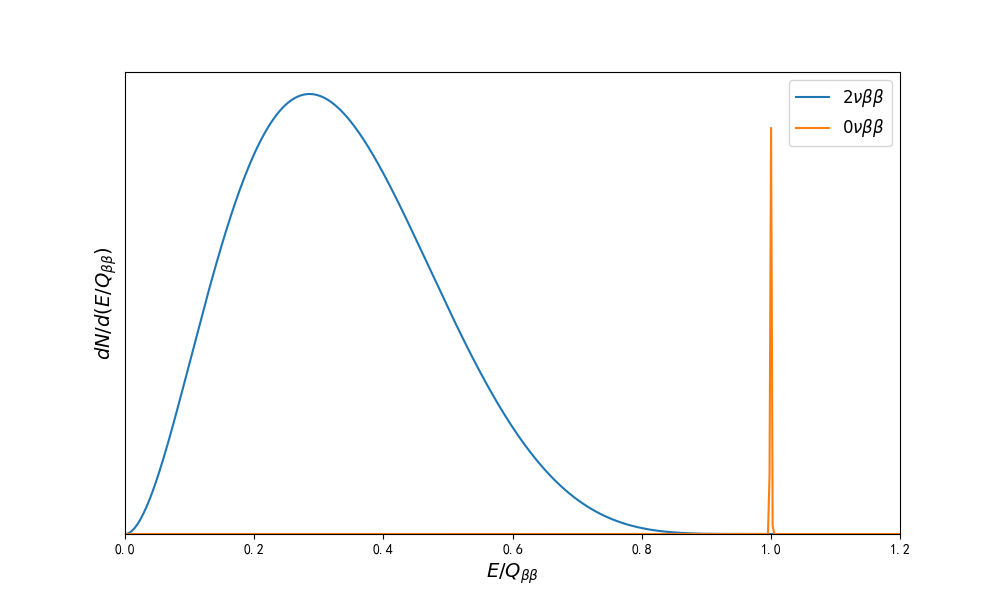
\includegraphics[width=0.9\textwidth]{figures/0vbb_2vbb.png}
    \caption{0$\nu\beta\beta$和2$\nu\beta\beta$衰变的能谱对比 (非真实比例)}
    \label{fig:0vbb_2vbb}
\end{figure}